% questions.tex —— 2013 年·天津卷·理科 · 题目内容片段（无答案）
% 由 tools/generate_projects.py 依来源总账自 2013/2013_数学真题_天津理_试题.md 生成，勿手改（改源 MD 后重跑）


\begin{gknotice}
\textbf{来源说明}：本题面依据固定源 PDF 的两页 A3 题面逐题转录，原卷印刷页码为 849–850，选择题 1—8、填空题 9—14、解答题 15—17 在第 849 面，解答题 18—20 在第 850 面；原卷无选做栏。

\textbf{解析归属}：固定源不附答案或解析；配套答案与解析均由本库按本题面独立复算。

\textbf{图形说明}：第 3 题程序框图、第 13 题圆内接三角形、第 17 题四棱柱图均由项目内 TikZ 矢量源重绘。
\end{gknotice}

\gkpart{一、选择题}

\begin{question}
\gkti{1}已知集合 $A=\{x\in\mathbf{R}\mid |x|\leqslant 2\}$，$B=\{x\in\mathbf{R}\mid x\leqslant 1\}$，则 $A\cap B=$\mbox{（　　）}

（A）$(-\infty,2]$；（B）$[1,2]$；（C）$[-2,2]$；（D）$[-2,1]$。

\end{question}
\begin{question}
\gkti{2}设变量 $x$，$y$ 满足约束条件
\nopagebreak[4]
\[\begin{cases}
3x+y-6\geqslant 0,\\
x-y-2\leqslant 0,\\
y-3\leqslant 0,
\end{cases}\]
则目标函数 $z=y-2x$ 的最小值为\mbox{（　　）}

（A）$-7$；（B）$-4$；（C）$1$；（D）$2$。

\Needspace{0.4\textheight}
\end{question}
\begin{question}
\gkti{3}阅读如图的程序框图，运行相应的程序，若输入 $x$ 的值为 $1$，则输出 $S$ 的值为\mbox{（　　）}
\nopagebreak[4]
\begin{center}% ============================================================
% f2013_tianjin_science_q03_flowchart.tex
% 2013 天津卷（理科）第 3 题 程序框图（TikZ 矢量重绘）
% 逻辑：输入 x → S=0 → S=S+x^3 → 判断 S>=50?
%       否 → x=2x → 回到 S=S+x^3；是 → 输出 S → 结束
% ============================================================
\begin{tikzpicture}[
  x=1cm, y=1cm, scale=0.8, transform shape,
  every node/.style={font=\small, inner sep=1pt},
  box/.style={draw, line width=0.6pt, minimum height=0.8cm, align=center},
  arr/.style={-{Stealth[length=2.4mm,width=1.8mm]}, line width=0.6pt},
]

  % ---------- 主干 ----------
  \draw[arr] (0,9.80) -- (0,9.02);
  \draw[arr] (0,8.18) -- (0,7.48);
  \draw[arr] (0,6.72) -- (0,5.92);
  \draw[arr] (0,5.10) -- (0,4.62);
  \draw[arr] (0,2.98) -- (0,2.22);
  \draw[arr] (0,1.38) -- (0,0.74);

  % ---------- 「否」支：菱形右顶点 → 右 → 上 → x=2x ----------
  \draw[arr] (2.90,3.80) -- (4.60,3.80) -- (4.60,5.88);

  % ---------- 回代：x=2x 左侧 → 左 → 下，汇入主干 ----------
  \draw[arr] (3.64,6.30) -- (0,6.30) -- (0,5.92);

  % ---------- 节点 ----------
  \node[box, rounded corners=4pt, minimum width=2.6cm] at (0,10.22) {开始};

  \draw[line width=0.6pt]
    (-1.80,8.18) -- (1.80,8.18) -- (1.42,9.02) -- (-1.42,9.02) -- cycle;
  \node at (0,8.60) {输入 $x$};

  \node[box, minimum width=2.2cm] at (0,7.10) {$S=0$};

  \node[box, minimum width=3.8cm] at (0,5.50) {$S=S+x^3$};

  \draw[line width=0.6pt]
    (0,4.62) -- (2.90,3.80) -- (0,2.98) -- (-2.90,3.80) -- cycle;
  \node at (0,3.80) {$S\geqslant 50$?};

  \draw[line width=0.6pt]
    (-1.70,1.38) -- (1.70,1.38) -- (1.38,2.22) -- (-1.38,2.22) -- cycle;
  \node at (0,1.80) {输出 $S$};

  \node[box, rounded corners=4pt, minimum width=2.4cm] at (0,0.34) {结束};

  \node[box, minimum width=1.9cm] at (4.60,6.30) {$x=2x$};

  % ---------- 分支标注 ----------
  \node at (0.34,2.58) {是};
  \node at (3.55,4.02) {否};

\end{tikzpicture}
\end{center}
\nopagebreak[4]
（A）$64$；（B）$73$；（C）$512$；（D）$585$。

\end{question}
\begin{question}
\gkti{4}已知下列三个命题：

① 若一个球的半径缩小到原来的 $\dfrac12$，则其体积缩小到原来的 $\dfrac18$；

② 若两组数据的平均数相等，则它们的标准差也相等；

③ 直线 $x+y+1=0$ 与圆 $x^2+y^2=\dfrac12$ 相切。

其中真命题的序号是\mbox{（　　）}

（A）①②③；（B）①②；（C）①③；（D）②③。

\end{question}
\begin{question}
\gkti{5}已知双曲线 $\dfrac{x^2}{a^2}-\dfrac{y^2}{b^2}=1$（$a>0$，$b>0$）的两条渐近线与抛物线 $y^2=2px$（$p>0$）的准线分别交于 $A$，$B$ 两点，$O$ 为坐标原点。若双曲线的离心率为 $2$，$\triangle AOB$ 的面积为 $\sqrt3$，则 $p=$\mbox{（　　）}

（A）$1$；（B）$\dfrac32$；（C）$2$；（D）$3$。

\end{question}
\begin{question}
\gkti{6}在 $\triangle ABC$ 中，$\angle ABC=\dfrac{\pi}{4}$，$AB=\sqrt2$，$BC=3$，则 $\sin\angle BAC=$\mbox{（　　）}

（A）$\dfrac{\sqrt{10}}{10}$；（B）$\dfrac{\sqrt{10}}{5}$；（C）$\dfrac{3\sqrt{10}}{10}$；（D）$\dfrac{\sqrt5}{5}$。

\end{question}
\begin{question}
\gkti{7}函数 $f(x)=2^x|\log_{0.5}x|-1$ 的零点个数为\mbox{（　　）}

（A）$1$；（B）$2$；（C）$3$；（D）$4$。

\end{question}
\begin{question}
\gkti{8}已知函数 $f(x)=x(1+a|x|)$。设关于 $x$ 的不等式 $f(x+a)<f(x)$ 的解集为 $A$，若 $\left[-\dfrac12,\dfrac12\right]\subseteq A$，则实数 $a$ 的取值范围是\mbox{（　　）}

（A）$\left(\dfrac{1-\sqrt5}{2},0\right)$；（B）$\left(\dfrac{1-\sqrt3}{2},0\right)$；（C）$\left(\dfrac{1-\sqrt5}{2},0\right)\cup\left(0,\dfrac{1+\sqrt3}{2}\right)$；（D）$\left(-\infty,\dfrac{1-\sqrt5}{2}\right)$。

\end{question}
\begingroup
\renewcommand{\gkpart}[1]{\Needspace{0.4\textheight}\subsection*{#1}\nopagebreak}
\gkpart{二、填空题}
\endgroup

\begin{question}
\gkti{9}已知 $a$，$b\in\mathbf{R}$，$\mathrm i$ 是虚数单位。若 $(a+\mathrm i)(1+\mathrm i)=b\mathrm i$，则 $a+b\mathrm i=$\gkblank{}。

\end{question}
\begin{question}
\gkti{10}$\left(x-\dfrac{1}{\sqrt{x}}\right)^6$ 的二项展开式中的常数项为\gkblank{}。

\end{question}
\begin{question}
\gkti{11}已知圆的极坐标方程为 $\rho=4\cos\theta$，圆心为 $C$，点 $P$ 的极坐标为 $\left(4,\dfrac{\pi}{3}\right)$，则 $|CP|=$\gkblank{}。

\end{question}
\begin{question}
\gkti{12}在平行四边形 $ABCD$ 中，$AD=1$，$\angle BAD=60^\circ$，$E$ 为 $CD$ 的中点。若 $\overrightarrow{AC}\cdot\overrightarrow{BE}=1$，则 $AB$ 的长为\gkblank{}。

\Needspace{0.4\textheight}
\end{question}
\begin{question}
\gkti{13}如图，$\triangle ABC$ 为圆的内接三角形，$BD$ 为圆的弦，且 $BD\parallel AC$。过点 $A$ 作圆的切线与 $DB$ 的延长线交于点 $E$，$AD$ 与 $BC$ 交于点 $F$。若 $AB=AC$，$AE=6$，$BD=5$，则线段 $CF$ 的长为\gkblank{}。
\nopagebreak[4]
\begin{center}% ============================================================
% f2013_tianjin_science_q13_circle.tex
% 2013 天津卷（理科）第 13 题 圆内接三角形与切线（TikZ 矢量重绘）
% 几何：圆 O，A 在圆上；AB=AC；BD∥AC，E 在 DB 延长线上，EA 切圆于 A；
%       AD 与 BC 交于 F。图中坐标按题设 AE=6、BD=5、AB=AC 精确构造后缩放。
% ============================================================
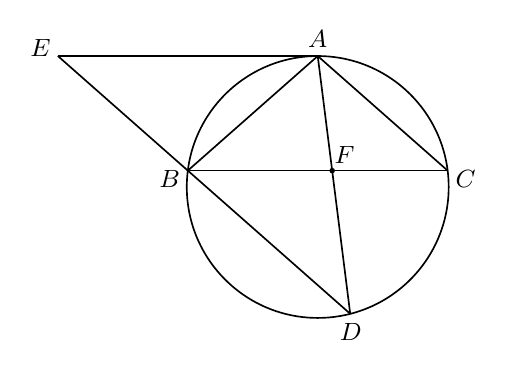
\begin{tikzpicture}[
  x=1cm, y=1cm,
  every node/.style={font=\small, inner sep=1pt},
  line/.style={line width=0.6pt},
]

  % 圆：R = 8/sqrt(7) * 0.55
  \draw[line] (0,0) circle [radius=1.6630];

  % 切线 EA 与割线 E-B-D
  \draw[line] (-3.30,1.6630) -- (0,1.6630);
  \draw[line] (-3.30,1.6630) -- (0.4125,-1.6105);

  % 三角形 ABC 与弦 AD
  \draw[line] (0,1.6630) -- (-1.6500,0.2078);
  \draw[line] (0,1.6630) -- (1.6500,0.2078);
  \draw[line] (-1.6500,0.2078) -- (1.6500,0.2078);
  \draw[line] (0,1.6630) -- (0.4125,-1.6105);

  % 交点 F
  \fill (0.1833,0.2078) circle [radius=0.035];

  % 标签
  \node at (0,1.88) {$A$};
  \node at (-1.88,0.10) {$B$};
  \node at (1.88,0.10) {$C$};
  \node at (0.42,-1.84) {$D$};
  \node at (-3.52,1.76) {$E$};
  \node at (0.34,0.40) {$F$};

\end{tikzpicture}
\end{center}
\nopagebreak[4]
\end{question}
\begin{question}
\gkti{14}设 $a+b=2$，$b>0$，则当 $a=$\gkblank{}时，$\dfrac{1}{2|a|}+\dfrac{|a|}{b}$ 取得最小值。

\end{question}
\begingroup
\renewcommand{\gkpart}[1]{\Needspace{0.4\textheight}\subsection*{#1}\nopagebreak}
\gkpart{三、解答题}
\endgroup

\begin{question}
\gkti{15}已知函数 $f(x)=-\sqrt2\sin\left(2x+\dfrac{\pi}{4}\right)+6\sin x\cos x-2\cos^2x+1$，$x\in\mathbf{R}$。

（1） 求 $f(x)$ 的最小正周期；

（2） 求 $f(x)$ 在区间 $\left[0,\dfrac{\pi}{2}\right]$ 上的最大值和最小值。

\end{question}
\begin{question}
\gkti{16}一个盒子里装有 7 张卡片，其中有红色卡片 4 张，编号分别为 1，2，3，4；白色卡片 3 张，编号分别为 2，3，4。从盒子中任取 4 张卡片（假设取到任何一张卡片的可能性相同）。

（1） 求取出的 4 张卡片中，含有编号为 3 的卡片的概率。

（2） 在取出的 4 张卡片中，红色卡片编号的最大值设为 $X$，求随机变量 $X$ 的分布列和数学期望。

\Needspace{0.4\textheight}
\end{question}
\begin{question}
\gkti{17}如图所示，在四棱柱 $ABCD\text{-}A_1B_1C_1D_1$ 中，侧棱 $A_1A\perp$ 底面 $ABCD$，$AB\parallel DC$，$AB\perp AD$，$AD=CD=1$，$AA_1=AB=2$，$E$ 为棱 $AA_1$ 的中点。

（1） 证明：$B_1C_1\perp CE$；

（2） 求二面角 $B_1\text{-}CE\text{-}C_1$ 的平面角的正弦值；

（3） 设点 $M$ 在线段 $C_1E$ 上，且直线 $AM$ 与平面 $ADD_1A_1$ 所成角的正弦值为 $\dfrac{\sqrt2}{6}$，求线段 $AM$ 的长。
\nopagebreak[4]
\begin{center}% ============================================================
% f2013_tianjin_science_q17_prism.tex
% 2013 天津卷（理科）第 17 题 四棱柱 ABCD-A1B1C1D1（TikZ 矢量重绘）
% 题设：A1A⊥底面 ABCD，AB∥DC，AB⊥AD，AD=CD=1，AA1=AB=2，
%       E 为 AA1 中点。底面为直角梯形，图中按斜二测投影绘制。
% 实线：可见棱；虚线：被遮挡棱与辅助线 AC、CE、EC1。
% ============================================================
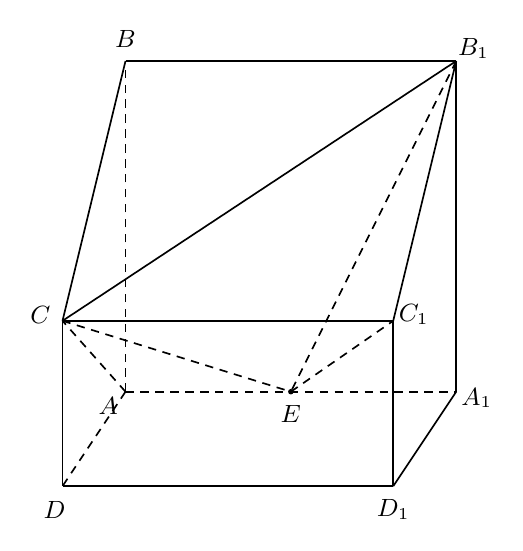
\begin{tikzpicture}[
  x=1cm, y=1cm,
  every node/.style={font=\small, inner sep=1pt},
  s/.style={line width=0.6pt},
  d/.style={line width=0.6pt, dash pattern=on 3.0pt off 2.4pt},
]

  % ---------- 实线 ----------
  \draw[s] (0,0) -- (0,2.10);          % D-C
  \draw[s] (0,2.10) -- (4.20,2.10);    % C-C1
  \draw[s] (4.20,2.10) -- (4.20,0);    % C1-D1
  \draw[s] (4.20,0) -- (0,0);          % D1-D

  \draw[s] (0,2.10) -- (0.80,5.40);    % C-B
  \draw[s] (0.80,5.40) -- (5.00,5.40); % B-B1
  \draw[s] (5.00,5.40) -- (4.20,2.10); % B1-C1
  \draw[s] (5.00,5.40) -- (5.00,1.20); % B1-A1
  \draw[s] (5.00,1.20) -- (4.20,0);    % A1-D1
  \draw[s] (5.00,5.40) -- (0,2.10);    % B1-C

  % ---------- 虚线 ----------
  \draw[d] (0.80,1.20) -- (0.80,5.40); % A-B
  \draw[d] (0.80,1.20) -- (0,0);       % A-D
  \draw[d] (0.80,1.20) -- (5.00,1.20); % A-A1（过 E）
  \draw[d] (0.80,1.20) -- (0,2.10);    % A-C
  \draw[d] (0,2.10) -- (2.90,1.20);    % C-E
  \draw[d] (2.90,1.20) -- (4.20,2.10); % E-C1
  \draw[d] (5.00,5.40) -- (2.90,1.20); % B1-E（原页辅助线）

  % E 点
  \fill (2.90,1.20) circle [radius=0.035];

  % ---------- 标签 ----------
  \node at (0.58,1.02) {$A$};
  \node at (0.80,5.68) {$B$};
  \node at (-0.28,2.18) {$C$};
  \node at (4.46,2.18) {$C_1$};
  \node at (-0.10,-0.30) {$D$};
  \node at (4.20,-0.30) {$D_1$};
  \node at (5.26,1.12) {$A_1$};
  \node at (5.22,5.56) {$B_1$};
  \node at (2.90,0.92) {$E$};

\end{tikzpicture}
\end{center}
\nopagebreak[4]
\end{question}
\begin{question}
\gkti{18}设椭圆 $\dfrac{x^2}{a^2}+\dfrac{y^2}{b^2}=1$（$a>b>0$）的左焦点为 $F$，离心率为 $\dfrac{\sqrt3}{3}$，过点 $F$ 且与 $x$ 轴垂直的直线被椭圆截得的线段长为 $\dfrac{4\sqrt3}{3}$。

（1） 求椭圆的方程；

（2） 设 $A$，$B$ 分别为椭圆的左、右顶点，过点 $F$ 且斜率为 $k$ 的直线与椭圆交于 $C$，$D$ 两点。若 $\overrightarrow{AC}\cdot\overrightarrow{DB}+\overrightarrow{AD}\cdot\overrightarrow{CB}=8$，求 $k$ 的值。

\end{question}
\begin{question}
\gkti{19}已知首项为 $\dfrac32$ 的等比数列 $\{a_n\}$ 不是递减数列，其前 $n$ 项和为 $S_n$（$n\in\mathbf{N}^{*}$），且 $S_3+a_3$，$S_5+a_5$，$S_4+a_4$ 成等差数列。

（1） 求数列 $\{a_n\}$ 的通项公式；

（2） 设 $T_n=S_n-\dfrac{1}{S_n}$（$n\in\mathbf{N}^{*}$），求数列 $\{T_n\}$ 的最大项的值与最小项的值。

\end{question}
\begin{question}
\gkti{20}已知函数 $f(x)=x^2\ln x$。

（1） 求函数 $f(x)$ 的单调区间；

（2） 证明：对任意的 $t>0$，存在唯一的 $s$，使 $t=f(s)$；

\Needspace{5\baselineskip}
（3） 设（2）中所确定的 $s$ 关于 $t$ 的函数为 $s=g(t)$，证明：当 $t>e^2$ 时，有
\nopagebreak[4]
\[\frac25<\frac{\ln g(t)}{\ln t}<\frac12.\]

\end{question}